% % \part{数学建模实战}
% % \chapter{证券收益率的GARCH族模型比较}


% %%%%%%%%%%%%%%%%%%%%%%%%%%%%%%%宋焱燚专用格式
% \documentclass[UTF8]{ctexbook}

% \ctexset{
%     part/number = \chinese{part}
% }
% \usepackage{multirow}
% \usepackage{amsmath}% ams 数学公式
% \usepackage{amsfonts}% ams 数学字体
% \usepackage{bbm}%重影字体
% \usepackage{amssymb,latexsym}% ams 数学符号与LaTeX数学符号
% \usepackage{mathrsfs}% 花式符号
% \usepackage{ntheorem}%定理、定义、证明
%   \theoremstyle{nonumberplain}
%   \theoremheaderfont{\bfseries}
%   \theorembodyfont{\normalfont}
%   \theoremsymbol{$\square$}
%   \newtheorem{Proof}{\hskip 2em 证明}
%   \newtheorem{theorem}{\hspace{2em}定理}[chapter]
%   \newtheorem{definition}{\hspace{2em}定义}[chapter] % 如果没有章, 只有节, 把上面的[chapter]改成[section]
%   \newtheorem{axiom}[definition]{\hspace{2em}公理}
%   \newtheorem{lemma}[definition]{\hspace{2em}引理}
%   \newtheorem{proposition}[definition]{\hspace{2em}命题}
%   \newtheorem{corollary}[definition]{\hspace{2em}推论}
%   \newtheorem{remark}{\hspace{2em}注}[chapter] %类似地定义其他“题头”. 这里“注”的编号与定义、定理等是分开的
%   \newtheorem{Assumption}{\hspace{2em}假设}[chapter]
% %算法伪代码
% \usepackage{algorithm}
% \usepackage{algorithmicx}
% \usepackage{algpseudocode}
%     \floatname{algorithm}{算法}
%     \renewcommand{\algorithmicrequire}{\textbf{输入:}}
%     \renewcommand{\algorithmicensure}{\textbf{输出:}}
% % 罗马数字:示例:\rom{2}
% \makeatletter
% \newcommand*{\rom}[1]{\expandafter\@slowromancap\romannumeral #1@}
% \makeatother

% \usepackage{enumerate}%itemiz环境。\begin{enumerate}[step 1][a)]可以使用 A,a,I,i,1 作为可选项产生
% \usepackage{cite}%参考文献
%     \bibliographystyle{plain}
% \usepackage{extarrows}% 带参数的箭头
% \usepackage{hyperref}% 超链接
% \usepackage{pifont}%然后在正文输入\ding{172}~\ding{211}得到相应数字,要是要①就输入:\ding{172}②就输:\ding{173}
% \hypersetup{
%     colorlinks=false,% 去掉超链接颜色
%     pdfborder=0 0 0% 取消超链接的边框
% }
% \usepackage{graphicx}% 图片管理
% % \usepackage{caption}
% % \usepackage{subcaption}%并排的图各有标题
% \graphicspath{{images/}}% 设置图片搜索路径
% \usepackage{float,varwidth}% 浮动体
% \usepackage{booktabs}% 三线表
% \usepackage{fancyhdr}% 页眉设置
% \usepackage{xcolor}% 颜色宏包
% \usepackage{colortbl}% 彩色表格
% \usepackage{listings}% 代码高亮
% \usepackage{caption}% 对标题进行控制,如让\caption标题的字体缩小一号,同时数字标签使用粗体可以用:\usepackage[font=small,labelfont=bf]{caption}
% % \usepackage{xfrac,upgreek}%分别是行间公式如a/b的形式(将原来的命令\frac改成\sfrac)和希腊字体的宏包的
% \usepackage{mathtools}%lgathered和rgathered环境把公式向左向右对齐
% % \usepackage{tabularx}%提供自动延伸的表列,(X列格式说明符),文字过长时可以自动转行
% % \usepackage{longtable}%长表格
% % \usepackage{enumitem}%enumerate宏包的升级
% % \usepackage{harpoon}%数学公式的矢量
% % \usepackage{bookmark}%目录的书签
% \renewcommand{\headwidth}{\textwidth}%图片并排,这个要列在所有宏包的后面
% \definecolor{codegreen}{rgb}{0,0.6,0}
% \definecolor{codegray}{rgb}{0.5,0.5,0.5}
% \definecolor{codepurple}{rgb}{0.58,0,0.82}
% \definecolor{backcolour}{rgb}{0.95,0.95,0.92}
% \lstset{
%     commentstyle=\color{codegreen},
%     keywordstyle=\color{magenta},
%     numberstyle=\tiny\color{codegray},
%     stringstyle=\color{codepurple},
%     basicstyle=\footnotesize,
%     breakatwhitespace=false,% 断行只在空格处
%     breaklines=true,% 自动断行
%     captionpos=b,% 标题位置
%     keepspaces=true,
%     numbers=left,
%     numbersep=5pt,
%     showspaces=false,
%     showstringspaces=false,
%     showtabs=false,% 显示
%     tabsize=2% TAB 被当作两个空格
% }
% \topmargin=0pt\oddsidemargin=0pt\evensidemargin=0pt
% \textwidth=16.5cm\textheight=23cm\raggedbottom%我这么设置是为了缩小页边距,满足有的文字无法转行
% % \pagestyle{headings}%页眉为章节标题,无页脚
% % \setlength{\abovecaptionskip}{10pt}
% % \setlength{\belowcaptionskip}{-15pt}%图片表格的前后距离设置
% % \CTEXsetup[format={\zihao{-3}\raggedright\bfseries}]{section}%设置节的格式
% \begin{document}
% \part{数学建模实战}
\chapter{证券收益率的GARCH族模型比较}

\section{背景}
    \par
    整本书都少有介绍时间序列模型,这是一个非常大的遗憾,因此,我们利用这章来简单的介绍一些时间序列模型\footnote{此部分主要是为了介绍各种GARCH模型}。
    在这一部分中,我们比较了ARMA和GARCH族模型在股票收益率上的建模效果。文中所有
    模型均为$p=1$和$q=1$的状态,所有模型均在正态分布下进行。利用FB收
    益率作为样本收益率进行分析,采用模型信息、残差检验以及模型拟合指标等方法评价各模型,并得到相应的结论。
    \par
    对股票收益率的建模一直以来都是统计与金融经济研究的重点。如果我们能够很好的描述收益率预估收益率,这将对我们今后的投资产生巨大的帮助,例如:我们可以在收益率模型的基础上建立组合投资模型,收益率的方差就是投资中的风险所在(这里,我们直接对收益率进行建模,因此说收益率即为误差项)。但不幸的是:收益率具有随机性、波动聚集性、杠杆效应和厚尾特征等特性,这使得我们很难建立好的模型来拟合收益率。经过前人们的不断努力,人们对收益率的认知越来越丰富,可以说每一个收益率都是一个独特的个体,每个个体有其自身的特性,而众多的收益率在一起,则表现出一些共性(随机性、杠杆效应、厚尾特征等等),因此,对收益率的建模会多种多样。既然对某个收益率而言,我们有如此多的模型可以选择,那么问题来了:就单一收益率而言,哪个模型更为合适?哪个模型适合大多数收益率?接下来的内容主要解决这第一个问题。我们选取某一收益率(FB收益率)进行分析,首先介绍ARMA和GARCH族模型,然后将模型应用到FB 上,最后进行模型的评价。值得一提的是:我们此次是在单一的FB时间序列上进行分析,后期,我们会扩展到一些多元时间序列模型。
\section{FB收益率序列基本分析}
    \subsection{FB收益率的描述统计}
        \par
        在进行收益率描述与建模之前,我们有必要设置一下符号。从yahoo财经上获取2014/05/22至2015/12/01的FB闭市股票数据,设$P_t$为$t$时刻的股票值,时长为$T$,设收益率为$x_t$
        \begin{equation*}
        x_{t}=\ln\left(\frac{P_t}{P_{t-1}}\right)
        \end{equation*}
        将收益率序列记为$\left\{x_t\right\}_{t=1}^T$,因为文中建立的是时间序列模型,所以,我们设定单一的$x_t$为随机变量,而$\left\{x_t\right\}$ 为随机过程,具体的$\left\{x_t\right\}$ 的值为随机过程的一次样本实现。
        \par
        我们先来描述一下$\left\{x_t\right\}$ 的统计特征,值得一提的是:本应该先对其进行平稳性分析,只有当$\left\{x_t\right\}$ 为平稳过程时,统计分析与建模才有意义。这里,我们将平稳性等检验放在后面进行。从2014/05/22开始,由于进行了差分运算,所以$\left\{x_t\right\}$ 从2014/05/23开始,对其进行基本统计分析,发现$\left\{x_t\right\}$ 最小收益率为-0.062716,最大收益率为0.050465,平均收益率为0.001483,绘制$\left\{x_t\right\}$ 的序列图如图(\ref{FB收益率序列图})所示
            \begin{figure}[H]
            \centering
            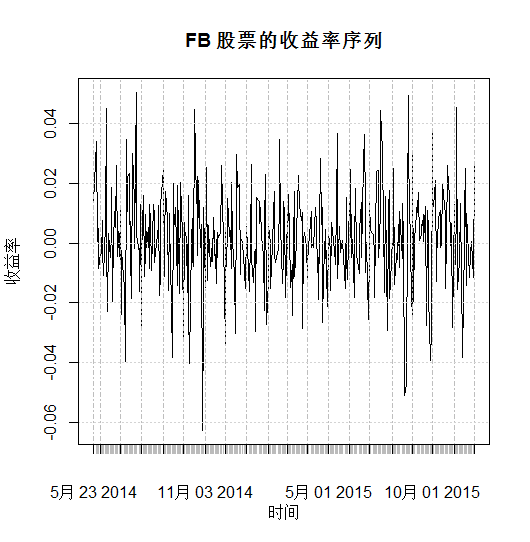
\includegraphics[width=6cm]{images/FB_rate_of_return.jpg}
            \caption{FB收益率序列图}
            \label{FB收益率序列图}
            \end{figure}
        发现收益率序列围绕0上下波动,并且具有一定的波动聚集性,表现为大的波动后面紧接大的波动。绘制$\left\{x_t\right\}$ 的序列直方图并进行非参数密度估计如图(\ref{收益率序列直方图及核密度估计})所示。
            \begin{figure}[H]
            \centering
            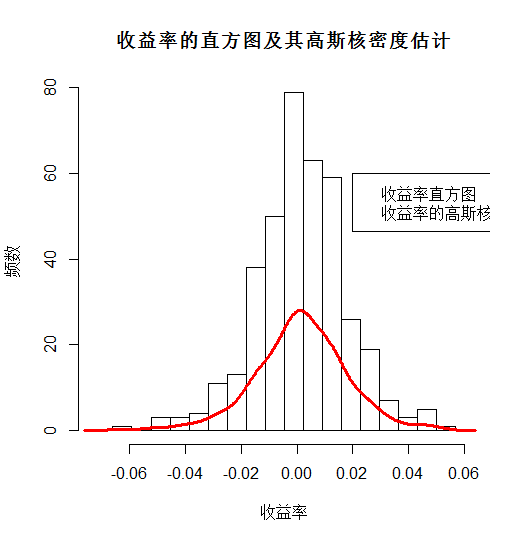
\includegraphics[width=6cm]{images/rate_of_return_sequence_nucear_density_estimation.jpg}
            \caption{收益率序列直方图及核密度估计}
            \label{收益率序列直方图及核密度估计}
            \end{figure}
        发现收益率序列具有一定的对称性,并且结合图(\ref{收益率序列直方图及核密度估计})和图(\ref{收益率序列QQ图}),我们可看到收益率序列相对正态分布而言具有厚尾的特点,并且在K-S检验下,收益率非正态。
            \begin{figure}[H]
            \centering
            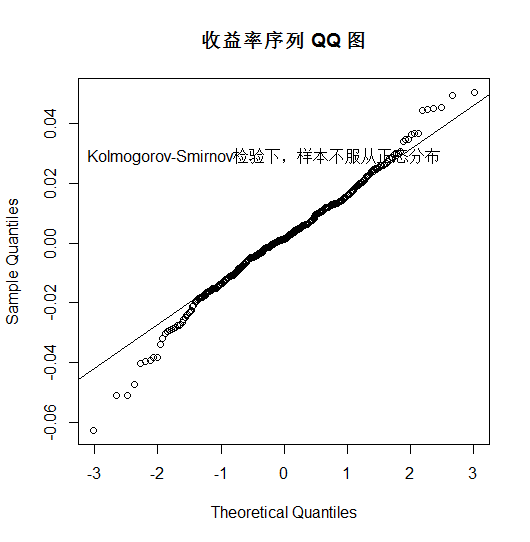
\includegraphics[width=6cm]{images/rate_of_return_sequence_QQ.jpg}
            \caption{收益率序列QQ图}
            \label{收益率序列QQ图}
            \end{figure}
        % \textcolor[rgb]{1 0 0}{todo:图片:收益率序列QQ图}
    \subsection{FB收益率的基本分析}
        \subsubsection{平稳性检验}
            \par
            序列具有平稳性是我们建立模型的前提(ARMA/GARCH均是在平稳序列上建立的模型),在平稳的条件下,我们才可以利用时间遍历性对序列进行分析,为此,我们先对$\left\{x_t\right\}$ (为便于书写,下面将$\left\{x_t\right\}$ 写为$x_t$ )进行平稳性检验。平稳性检验有许多方法,例如:非参数的游程检验法,ADF单位根检验法,PP(Phillips-Perron)检验法(R-uroot-pp.test)等。我们利用ADF 单位根检验来检验$x_t$ 的平稳性,ADF有三种检验类型:无常数无趋势$^1$、
            有常数无趋势$^2$、有常数有趋势$^3$。具体内容可参见一般时间序列教材(如:《应用时间序列分析》王黎明P232)。三种ADF检验的结果如表(\ref{收益率序列的三种ADF检验})所示。
            % \textcolor[rgb]{1.00,0.00,0.00}{todo:表格:收益率序列的三种ADF检验}
        \begin{table}[H]
        \centering
        \caption{收益率序列的三种ADF检验}
        \label{收益率序列的三种ADF检验}
        \begin{tabular}{lll}
            \toprule
            % 命令 & 函数说明&命令 & 函数说明\\
        % \midrule
    Test regression none$^1$   & p-value: < 2.2e-16  & Value of test-statistic is: -14.745\\
    Test regression drift$^2$  & p-value: < 2.2e-16  & Value of test-statistic is: -14.872\\
    Test regression trend$^3$  & p-value: < 2.2e-16  & Value of test-statistic is: -14.851\\
        \bottomrule
        \end{tabular}
        \end{table}
            \par
            经过ADF检验后,发现其$P$值$<0.05$,在0.05的显著水平下拒绝原假设,原假设为有一个单位根(非平稳),可以说明$x_t$为平稳时间序列。
        \subsubsection{相关性检验}
            \par
            相关性检验是重要的。如果序列不具有相关性,或者说序列为纯随机序列,那么我们也就没有建模的必要,接下来进行的相关性检验是线性相关性检验。利用Ljung-Box和Box-Pierce进行相关性检验,原假设假设序列为纯随机序列,检验后发现在0.05 的显著水平下拒绝原假设,序列$x_t$具有一定相关性。
            % \textcolor[rgb]{1.00,0.00,0.00}{todo:表}
            绘制收益率序列的自相关和偏自相关图,如图(\ref{收益率自相关偏自相关图})所示。
            \begin{figure}[H]
            \centering
            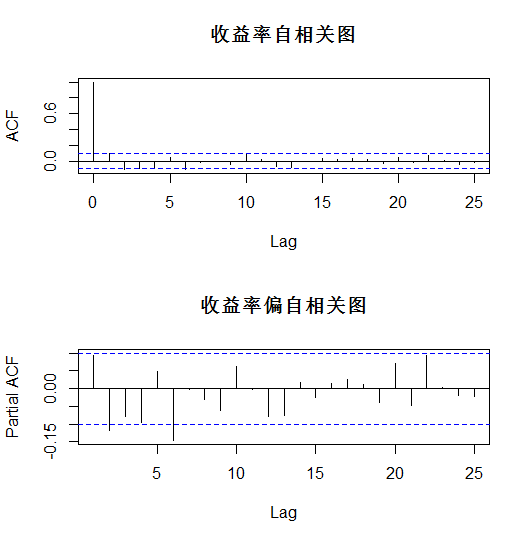
\includegraphics[width = 6cm]{images/rate_of_return_autocorrelation_partial_autocorrelation.jpg}
            \caption{收益率自相关偏自相关图}
            \label{收益率自相关偏自相关图}
            \end{figure}
            % \textcolor[rgb]{1.00,0.00,0.00}{todo:图片:收益率自相关偏自相关图}
        \subsubsection{ARCH检验}
            \par
            下面,我们将进行收益率序列的ARCH效应检验。ARCH效应的检验方法有许多,例如:LM(拉格朗日乘数检验)、McLead-Li-Test等,ARCH 说明收益率具有波动聚集的特点,我们先来绘制$x_t^2$的序列图及其自相关偏自相关图,如图(\ref{收益率序列平方的自相关偏自相关图})所示。可以发现,相对于$x_t$而言,其平方序列$x_t^2$具有更强的相关性,并且波动聚集明显。
            \begin{figure}[H]
            \centering
            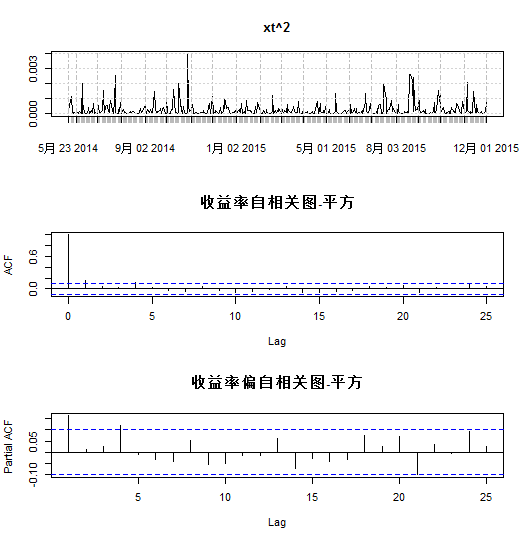
\includegraphics[width = 6cm]{images/rate_of_return_square_autocorrelation_partial_autocorrelation.jpg}
            \caption{收益率序列平方的自相关偏自相关图}
            \label{收益率序列平方的自相关偏自相关图}
            \end{figure}
            我们对$x_t$序列进行ARCH效应检验,先进行LMtest检验,检验原假设为$x_t$无ARCH效应,检验的滞后期为4、8和12(这是时间序列可能存在的周期),得到的检验结果如表(\ref{收益率序列的ARCH效应检验})所示。
            \begin{table}[H]
            \centering
            \caption{收益率序列的ARCH效应检验}
            \label{收益率序列的ARCH效应检验}
            \begin{tabular}{lll}
                \toprule
                % 命令 & 函数说明&命令 & 函数说明\\
            \multicolumn{3}{l}{ARCH LM-test, Null hypothesis: no ARCH effects}\\
            \midrule
            Chi-squared = 16.44 &df = 4 & p-value = 0.00248\\
            Chi-squared = 18.21 &df = 8 & p-value = 0.01971\\
            Chi-squared = 22.444&df = 12& p-value = 0.03283\\
            \bottomrule
            \end{tabular}
            \end{table}
            % \textcolor[rgb]{1.00,0.00,0.00}{todo:表格:收益率序列的ARCH效应检验}\\
            利用 McLead-Li-Test进行检验,检验原假设为$x_t$无ARCH效应,得到的检验结果如图(\ref{少收益率序列的McLead-Li ARCH 效应检验结果图})所示。二者的结果说明收益率序列$x_t$具有ARCH效应。
            \begin{figure}[H]
            \centering
            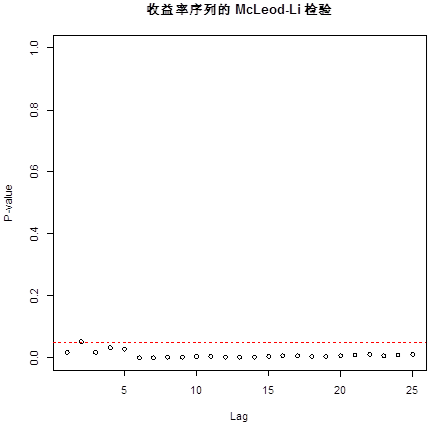
\includegraphics[width = 6cm]{images/McLead_Li_ARCH.png}
            \caption{少收益率序列的McLead-Li ARCH 效应检验结果图}
            \label{少收益率序列的McLead-Li ARCH 效应检验结果图}
            \end{figure}
\section{FB收益率的GARCH族模型建模}
    \par
    在收益率序列平稳的基础上对其进行建模,建立的模型主要是ARMA和GARCH 族,为简单,将所有模型统一建立为$(p,q)=(1,1)$,模型扰动项$\varepsilon_t$服从条件正态分布,为
    \[{\eta _t} \sim N(0,1),{\varepsilon _t}|{\Phi _t} \sim N(0,\sigma _t^2)\]
    当然,扰动项可以服从其它分布,例如:t分布,学生t以及广义误差分布GED等。分布不同,估计的极大似然不同,模型结果也就不同,因此,我们可以比较不同分布下的模型优良,但此问题并非我们所要讨论的。由于有不同的分布,我们在下面的模型介绍中,将其统一记为
    \[{\eta _t} \sim f,{\varepsilon _t}|{\Phi _t} \sim f(\sigma _t^2)\]
    \subsection{ARMA}
        \par
        Box and Jenkins于1970年撰写的《Time Series Analysis:Forecasting and Control》是时间序列发展的里程碑。
        ARMA的一般模型如下:
        \begin{equation*}
        \centering
        \left\{\begin{lgathered}
        {x_t} = c + \sum\limits_{i = 1}^p {{\phi _i}{x_{t - i}}}  + {\varepsilon _t} - \sum\limits_{j = 1}^q {{\varphi _j}{\varepsilon _{t - j}}} \\
        {\varepsilon _t} \sim WN(0,{\sigma ^2})
        \end{lgathered} \right.
        \end{equation*}
        我们在文中对$x_t$建立了ARMA(1,1)模型,ARMA(1,1)为
        \begin{equation*}
        \centering
        \left\{\begin{lgathered}
        {x_t} = c + {\phi _1}{x_{t - 1}} + {\varepsilon _t} - {\varphi _1}{\varepsilon _{t - 1}}\\
        {\varepsilon _t} \sim WN(0,{\sigma ^2})\\
        E({X_s},{\varepsilon _t}) = 0,\forall s < t
        \end{lgathered} \right.
        \end{equation*}
    \subsection{GARCH}
        收益率序列存在厚尾现象、波动聚集现象以及变方差(异方差)现象,Engle于1982年首先构建了ARCH模型用于刻画英国通货膨胀率中存在的异方差,他假设模型的残差$\varepsilon_t$的平方$\varepsilon_t^2$服从AR(p)过程,并且提出了检验序列是否具有ARCH效应的LM检验(Lagrange乘数法),具体内容可参见一般时间序列教材(如:《应用时间序列分析》王黎明P199)。Bollerslev于1986年将ARCH推广到一般的GARCH,GARCH与ARMA有类似的结构。
        \par
        GARCH模型的条件方差$\sigma_t^2$取决于残差$\varepsilon _{(t-i)}$的大小而与符号无关,但研究表明,收益率序列存在一定的杠杆效应,坏消息导致的价格波动要比好消息强烈。为了保证$\sigma_t^2$非负,要求模型系数为非负。GARCH 一般比较小,很难判断方差波动源的持续性。GARCH的一般模型如下:
        \begin{equation*}
        \centering
        \left\{\begin{lgathered}
        {x_t} = L(x) + {\varepsilon _t}\\
        {\varepsilon _t} = {\sigma _t}{\eta _t}\\
        \sigma _t^2 = w + \sum\limits_{i = 1}^q {{\alpha _i}\varepsilon _{t - i}^2}  + \sum\limits_{j = 1}^p {{\beta _j}\sigma _{t - j}^2} \\
        {\eta _t} \sim f,{\varepsilon _t}|{\Phi _t} \sim f(\sigma _t^2)
        \end{lgathered} \right.
        \end{equation*}
        其中,$L(x)$表示对序列$x_t$的任意模型,由于我们这里考虑的是单一时间序列建模,因此,也要求$L(x)$不受其他因素影响。
        \par
        我们在文中对$x_t$建立了GARCH(1,1)模型,GARCH(1,1)为
        \begin{equation*}
        \centering
        \left\{\begin{lgathered}
        {x_t} = c + {\varepsilon _t}\\
        {\varepsilon _t} = {\sigma _t}{\eta _t}\\
        \sigma _t^2 = w + {\alpha _1}\varepsilon _{t - 1}^2 + {\beta _1}\sigma _{t - 1}^2\\
        {\eta _t} \sim f,{\varepsilon _t}|{\Phi _t} \sim f(\sigma _t^2)
        \end{lgathered} \right.
        \end{equation*}
    \subsection{IGARCH}
        Bollerslev于1986年给出$\varepsilon_t$满足$garch(p,q)$的充要条件:
        \[{\varepsilon _t} \sim garch(p,q) \Leftrightarrow \sum\limits_{i = 1}^q {{\alpha _i}}  + \sum\limits_{j = 1}^p {{\beta _j}} < 1\]
        IGARCH是单位根GARCH,其在普通GARCH模型后面引入了约束,要求
        \[\sum\limits_{i = 1}^q {{\alpha _i}}  + \sum\limits_{j = 1}^p {{\beta _j}}  = 1\]
        这表明收益率具有强的持续的波动,这种情况下,条件方差函数具有单位根和单整性,任何对条件方差$\sigma_t^2$ 的影响都将持续下去。Bollerslev和Engle在1986年直接使用了IGARCH,但这种约束会使得真实的动态相依性变得有些强加的味道。IGARCH的一般模型如下
        \begin{equation*}
        \centering
        \left\{\begin{lgathered}
        {x_t} = L(x) + {\varepsilon _t}\\
        {\varepsilon _t} = {\sigma _t}{\eta _t}\\
        \sigma _t^2 = w + \sum\limits_{i = 1}^q {{\alpha _i}\varepsilon _{t - i}^2}  + \sum\limits_{j = 1}^p {{\beta _j}\sigma _{t - j}^2} \\
        \sum\limits_{i = 1}^q {{\alpha _i}}  + \sum\limits_{j = 1}^p {{\beta _j}}  = 1
        \end{lgathered} \right.
        \end{equation*}
        我们在论文中对$x_t$建立了IGARCH(1,1)模型,IGARCH(1,1)为
        \begin{equation*}
        \centering
        \left\{\begin{lgathered}
        {x_t} = c + {\varepsilon _t}\\
        {\varepsilon _t} = {\sigma _t}{\eta _t}\\
        \sigma _t^2 = w + {\alpha _1}\varepsilon _{t - 1}^2 + {\beta _1}\sigma _{t - 1}^2\\
        {\alpha _1} + {\beta _1} = 1
        \end{lgathered} \right.
        \end{equation*}
    \subsection{GARCHM}
        收益和波动率关系的非对称性归因于波动率的反馈效应,Engle、Lilien和Robin于1987年提出GARCHM模型来刻画这种非对称性,在模型中,条件均值显性的依赖于条件方差$\sigma_t^2$,表明当风险越大时,期望得到的收益也就越大。GARCHM的一般模型如下
        \begin{equation*}
        \centering
        \left\{\begin{lgathered}
        {x_t} = L(x) + {\varepsilon _t} + \gamma \sigma _t^2\\
        {\varepsilon _t} = {\sigma _t}{\eta _t}\\
        \sigma _t^2 = w + \sum\limits_{i = 1}^q {{\alpha _i}\varepsilon _{t - i}^2}  + \sum\limits_{j = 1}^p {{\beta _j}\sigma _{t - j}^2} \\
        {\eta _t} \sim f,{\varepsilon _t}|{\Phi _t} \sim f(\sigma _t^2)
        \end{lgathered} \right.
        \end{equation*}
        其中,$\gamma$ 称为风险溢价参数,$\gamma $为正时,表明高风险带来高收益。也有文献将风险标记为$\log⁡(\sigma_t^2)$。

        我们在论文中对$x_t$建立了GARCHM(1,1)模型,GARCHM(1,1)为

        \begin{equation*}
        \centering
        \left\{\begin{lgathered}
        {x_t} = c + {\varepsilon _t} + \gamma \sigma _t^2\\
        {\varepsilon _t} = {\sigma _t}{\eta _t}\\
        \sigma _t^2 = w + {\alpha _1}\varepsilon _{t - 1}^2 + {\beta _1}\sigma _{t - 1}^2\\
        {\alpha _1} + {\beta _1} = 1\\
        {\eta _t} \sim f,{\varepsilon _t}|{\Phi _t} \sim f(\sigma _t^2)
        \end{lgathered} \right.
        \end{equation*}
    \subsection{EGARCH}
        前面,我们提到过GARCH模型可以刻画收益率的异方差性,但其不能很好的表达收益率的杠杆效应,GARCH 模型的干扰因素$\eta_t$对条件方差的影响是对称的,不适合描述干扰对收益率的非对称影响,为了反应波动的非对称性,Nelson于1991年提出了指数GARCH模型(EGARCH),在模型中考虑了加权信息。
        \[g({\eta _t}) = \theta {\eta _t} + \gamma [\left| {{\eta _t}} \right| - E(\left| {{\eta _t}} \right|)]\]
        其中:$\theta$ 和$\gamma $是实常数,$\eta_t$是均值为0的独立同分布序列(过程),一般为正态白噪声,如果是正态白噪声,那么有$E\left(|\eta_t |\right)=\sqrt{2⁄\pi}$,并且:
        \[E\left[ {g\left( {{\eta _t}} \right)} \right] = 0\]
        $g(\eta_t )$的非对称性表现为
        \[g\left( {{\eta _t}} \right) = \left\{ \begin{array}{l}
        \left( {\theta  + \gamma } \right){\eta _t} - \gamma E\left( {\left| {{\eta _t}} \right|} \right),{\eta _t} \ge 0\\
        \left( {\theta  - \gamma } \right){\eta _t} - \gamma E\left( {\left| {{\eta _t}} \right|} \right),{\eta _t} \le 0
        \end{array} \right.\]
        一般的EGARCH模型如下:
        \begin{equation*}
        \centering
        \left\{\begin{lgathered}
        {x_t} = L(x) + {\varepsilon _t}\\
        {\varepsilon _t} = {\sigma _t}{\eta _t}\\
        \log \sigma _t^2 = w + \sum\limits_{i = 1}^q {{\alpha _i}g({\eta _{t - i}})}  + \sum\limits_{j = 1}^p {{\beta _j}\log \sigma _{t - j}^2} \\
        g({\eta _t}) = \theta {\eta _t} + \gamma [\left| {{\eta _t}} \right| - E(\left| {{\eta _t}} \right|)]
        \end{lgathered} \right.
        \end{equation*}
        \par
        我们在论文中对$x_t$建立了EGARCH (1,1)模型,EGARCH (1,1)为
        \begin{equation*}
        \centering
        \left\{\begin{lgathered}
        {x_t} = c + {\varepsilon _t}\\
        {\varepsilon _t} = {\sigma _t}{\eta _t}\\
        \log \sigma _t^2 = w + {\alpha _1}\left(\theta \frac{{{\varepsilon _{t - 1}}}}{{{\sigma _{t - 1}}}} + \gamma \left[\left| {\frac{{{\varepsilon _{t - 1}}}}{{{\sigma _{t - 1}}}}} \right| - E\left(\left| {\frac{{{\varepsilon _{t - 1}}}}{{{\sigma _{t - 1}}}}} \right|\right)\right]\right) + {\beta _1}\log \sigma _{t - 1}^2\\
        E\left(\left| {\frac{{{\varepsilon _{t - 1}}}}{{{\sigma _{t - 1}}}}} \right|\right) = \sqrt {2/\pi } ,\quad if\quad {\eta _t} \sim N(0,1)
         \end{lgathered} \right.
         \end{equation*}
    \subsection{GJRGARCH}
        另一个经常用来处理杠杆效应的模型是门限GARCH模型,这里,我们先来介绍GJRGARCH模型,然后介绍TGARCH模型,二者本质上是一样的。Glosten、Jagannathan和Runkle于1993年构建了GJRGARCH,他们在模型中引入了特征变量:
        \[{I_{t - i}} = 1({\varepsilon _{t - i}} < 0)\]
        当$\varepsilon_{(t-i)}<0$时,$I_{(t-i)}=1$,否则为0。GJRGARCH的一般模型如下:
        \begin{equation*}
        \centering
        \left\{\begin{lgathered}
        {x_t} = L(x) + {\varepsilon _t}\\
        {\varepsilon _t} = {\sigma _t}{\eta _t}\\
        \sigma _t^2 = w + \sum\limits_{i = 1}^q {\left( {{\alpha _i} + {\gamma _i}{I_{t - i}}} \right)\varepsilon _{t - i}^2}  + \sum\limits_{j = 1}^p {{\beta _j}\sigma _{t - j}^2} \\
        {I_{t - i}} = 1({\varepsilon _{t - i}} < 0)
         \end{lgathered} \right.
         \end{equation*}
        其中:$\alpha_i$,$\beta_i$和$\gamma_i$为非负参数,可以看到,正的$\varepsilon_{(t-i)}$对$\sigma_t$的贡献为$\alpha_i \varepsilon_{(t-i)}^2$,而负的$\varepsilon_{(t-i)} $对$\sigma_t$ 的贡献为$\left(\alpha_i +\gamma_i\right)\varepsilon_{(t-i)}^2$。
        \par
        我们在文中对$x_t$建立了GJRGARCH (1,1)模型,GJRGARCH (1,1)为:
        \begin{equation*}
        \centering
        \left\{\begin{lgathered}
        {x_t} = c + {\varepsilon _t}\\
        {\varepsilon _t} = {\sigma _t}{\eta _t}\\
        \sigma _t^2 = w + \left( {{\alpha _1} + {\gamma _1}{I_{t - 1}}} \right)\varepsilon _{t - 1}^2 + {\beta _1}\sigma _{t - 1}^2\\
        {I_{t - i}} = 1({\varepsilon _{t - i}} < 0)
        \end{lgathered} \right.
         \end{equation*}
    \subsection{TGARCH}
        Zakian于1994年提出门限GARCH模型,和GJRGARCH模型具有异曲同工之妙,不过,相对于GJRGARCH而言TGARCH有更少的参数。一般的TGARCH模型如下:
        \begin{equation*}
        \centering
        \left\{\begin{lgathered}
        {x_t} = L(x) + {\varepsilon _t}\\
        {\varepsilon _t} = {\sigma _t}{\eta _t}\\
        \sigma _t^2 = w + \sum\limits_{i = 1}^q {{\alpha _i}\varepsilon _{t - i}^2}  + \gamma {I_{t - i}}\varepsilon _{t - i}^2 + \sum\limits_{j = 1}^p {{\beta _j}\sigma _{t - j}^2} \\
        {I_{t - i}} = 1({\varepsilon _{t - i}} < 0)
        \end{lgathered} \right.
         \end{equation*}
         \par
        我们在文中对$x_t$建立了TGARCH (1,1)模型,TGARCH (1,1)为:
        \begin{equation*}
        \centering
        \left\{\begin{lgathered}
        {x_t} = c + {\varepsilon _t}\\
        {\varepsilon _t} = {\sigma _t}{\eta _t}\\
        \sigma _t^2 = w + {\alpha _1}\varepsilon _{t - 1}^2 + \gamma {I_{t - 1}}\varepsilon _{t - 1}^2 + {\beta _1}\sigma _{t - 1}^2\\
        {I_{t - i}} = 1({\varepsilon _{t - i}} < 0)
         \end{lgathered} \right.
         \end{equation*}
    \subsection{AGARCH and avGARCH}
        另一个用来刻画杠杆效应的有效模型是AGARCH(an asymeetric GARCH),AGARCH模型中引入了控制参数$b$,具体的AGARCH模型如下:
        \begin{equation*}
        \centering
        \left\{\begin{lgathered}
        {x_t} = L(x) + {\varepsilon _t}\\
        {\varepsilon _t} = {\sigma _t}{\eta _t}\\
        \sigma _t^2 = w + \sum\limits_{i = 1}^q {{\alpha _i}{{\left| {{\varepsilon _{t - i}} + b} \right|}^2}}  + \sum\limits_{j = 1}^p {{\beta _j}\sigma _{t - j}^2} \\
        {\eta _t} \sim f,{\varepsilon _t}|{\Phi _t} \sim f(\sigma _t^2)
        \end{lgathered} \right.
         \end{equation*}
        可以看到,当控制参数$b<0$时,负的$\varepsilon_{(t-i)}$对条件方差的贡献增大,正的$\varepsilon_{(t-i)}$对条件方差的贡献减小。
        \par
        一个扩展后的模型是avGARCH(absolute value GARCH),一般的avGARCH模型如下:
        \begin{equation*}
        \centering
        \left\{\begin{lgathered}
        {x_t} = L(x) + {\varepsilon _t}\\
        {\varepsilon _t} = {\sigma _t}{\eta _t}\\
        \sigma _t^2 = w + \sum\limits_{i = 1}^q {{\alpha _i}{{\left( {\left| {{\varepsilon _{t - i}} + b} \right| - c\left( {{\varepsilon _{t - i}} + b} \right)} \right)}^2}}  + \sum\limits_{j = 1}^p {{\beta _j}\sigma _{t - j}^2} \\
        {\eta _t} \sim f,{\varepsilon _t}|{\Phi _t} \sim f(\sigma _t^2)
        \end{lgathered} \right.
         \end{equation*}
    \subsection{nGARCH}
        Duan于1995年构建了NGARCH模型,用于刻画收益率的杠杆效应,同时反应了波动率的非线性性。一般的NGARCH模型如下:
        \begin{equation*}
        \centering
        \left\{\begin{lgathered}
        {x_t} = L(x) + \lambda {\sigma _t} - {\raise0.5ex\hbox{$\scriptstyle 1$}
        \kern-0.1em/\kern-0.15em
        \lower0.25ex\hbox{$\scriptstyle 2$}}\sigma _t^2 + {\varepsilon _t}\\
        {\varepsilon _t} = {\sigma _t}{\eta _t}\\
        \sigma _t^2 = w + \sum\limits_{i = 1}^q {{\alpha _i}{{\left( {{\varepsilon _{t - i}} - \lambda {\sigma _{t - j}}} \right)}^2}}  + \sum\limits_{j = 1}^p {{\beta _j}\sigma _{t - j}^2} \\
        {\eta _t} \sim f,{\varepsilon _t}|{\Phi _t} \sim f(\sigma _t^2)
         \end{lgathered} \right.
         \end{equation*}
        其中:参数$\lambda$用于刻画杠杆效应,如果其估计值非负,则说明具有杠杆效应。模型中的其他系数保持非负特点。
        \par
        我们在文中对$x_t$建立了NGARCH (1,1)模型,NGARCH (1,1)为:
        \begin{equation*}
        \centering
        \left\{\begin{lgathered}
        {x_t} = c + \lambda {\sigma _t} - {\raise0.5ex\hbox{$\scriptstyle 1$}
        \kern-0.1em/\kern-0.15em
        \lower0.25ex\hbox{$\scriptstyle 2$}}\sigma _t^2 + {\varepsilon _t}\\
        {\varepsilon _t} = {\sigma _t}{\eta _t}\\
        \sigma _t^2 = w + {\alpha _1}{\left( {{\varepsilon _{t - 1}} - \lambda {\sigma _{t - 1}}} \right)^2} + {\beta _1}\sigma _{t - 1}^2\\
        {\eta _t} \sim f,{\varepsilon _t}|{\Phi _t} \sim f(\sigma _t^2)
         \end{lgathered} \right.
         \end{equation*}
    \subsection{apARCH}
        Ding Z, G ranger C W J和Engle R F于1993年提出非对称幂GARCH(apARCH),apARCH仍然是用来刻画收益率的杠杆效应,并且,许多其他的模型可以从apARCH模型中演化形成,一般的apARCH模型如下:
        \begin{equation*}
        \centering
        \left\{\begin{lgathered}
        {x_t} = L(x) + {\varepsilon _t}\\
        {\varepsilon _t} = {\sigma _t}{\eta _t}\\
        \sigma _t^2 = w + \sum\limits_{i = 1}^q {{\alpha _i}{{\left( {\left| {{\varepsilon _{t - i}}} \right| - {\gamma _i}{\varepsilon _{t - i}}} \right)}^\delta }}  + \sum\limits_{j = 1}^p {{\beta _j}\sigma _{t - j}^\delta } \\
        {\eta _t} \sim f,{\varepsilon _t}|{\Phi _t} \sim f(\sigma _t^2)
         \end{lgathered} \right.
         \end{equation*}
        其中:$\gamma_i$用于刻画杠杆效应,当其为正时,表明具有杠杆效应。$\delta$为幂参数,当$\delta=1$时,模型变为TGARCH。
        \par
        我们在文中对$x_t$建立了apARCH (1,1)模型,apARCH (1,1)为:
        \begin{equation*}
        \centering
        \left\{\begin{lgathered}
        {x_t} = c + {\varepsilon _t}\\
        {\varepsilon _t} = {\sigma _t}{\eta _t}\\
        \sigma _t^2 = w + {\alpha _1}{\left( {\left| {{\varepsilon _{t - 1}}} \right| - {\gamma _1}{\varepsilon _{t - 1}}} \right)^\delta } + {\beta _1}\sigma _{t - 1}^\delta \\
        {\eta _t} \sim f,{\varepsilon _t}|{\Phi _t} \sim f(\sigma _t^2)
         \end{lgathered} \right.
         \end{equation*}
\section{模型估计与模型信息}
    \par
    在展示模型估计结果之前,要说明的是我们使用的是ruGARCH和bayesGARCH等R包,包中的模型和上面给出的标准模型可能会有一定的差异,具体的模型可以参考ruGARCH包的说明文档。一个普遍存在的差异是,ruGARCH包中的GARCH族模型的异方差模型为:
    \[\sigma _t^2 = \left( {w + \sum\limits_{j = 1}^m {{\zeta _j}{\nu _{jt}}} } \right) + \sum\limits_{i = 1}^q {{\alpha _i}{f_1}\left( {{\varepsilon _{t - i}}} \right)}  + \sum\limits_{j = 1}^p {{\beta _j}{f_2}\left( {{\sigma _{t - j}}} \right)} \]
    其常数项已经不再是常数项,在估计结果中,将$\zeta_j$记为omega。
    \par
    接下来我们直接给出模型的估计结果及模型的信息,不写出详细模型,最后给出各个模型的比较。
    \par
    1、ARMA模型参数估计结果如表(\ref{ARMA模型参数估计结果})所示
        \begin{table}[H]
        \centering
        \caption{ARMA模型参数估计结果}
        \label{ARMA模型参数估计结果}
        \begin{tabular}{lllll}
            \toprule
            Coefficient(s)&  Estimate  &  Std.Error & $t$ value & Pr(>|t|)\\
        \midrule
        ar1& -0.6374947 & 0.1377807 &  -4.627 & 3.71e-06***\\
        ma1& 0.7517159  & 0.1162311 &  6.467  & 9.97e-11***\\
        mu & 0.0014866  & 0.0008898 &  1.671  & 0.0948.\\
        \bottomrule
        \multicolumn{5}{l}{\footnotesize note: Signif. codes: 0 ‘***’ 0.001 ‘**’ 0.01 ‘*’ 0.05 ‘.’ 0.1 ‘ ’ 1;}\\
        \multicolumn{5}{l}{\footnotesize log likelihood: 1038.66 Distribution is:norm AIC Criterion: -2069.31}\\
        \end{tabular}
        \end{table}
    % \textcolor[rgb]{1.00,0.00,0.00}{todo:表格:ARMA模型参数估计结果}
    \par
    2、GARCH模型参数估计结果如表(\ref{GARCH模型参数估计结果})所示
        \begin{table}[H]
        \centering
        \caption{GARCH模型参数估计结果}
        \label{GARCH模型参数估计结果}
        \begin{tabular}{lllll}
            \toprule
            Coefficient(s)&  Estimate  &  Std.Error & $t$ value & Pr(>|t|)\\
        \midrule
        omega  & 0.0002188  & 0.0001091 &  2.005 &  0.0450*\\
        alpha1 & 0.1265543  & 0.0633417 &  1.998 &  0.0457*\\
        beta1  & 0.0703620  & 0.4113794 &  0.171 &  0.8642 \\
        \bottomrule
        \multicolumn{5}{l}{\footnotesize Log Likelihood:1037.195; normalized: 2.694013 Conditional Distribution is:norm.}\\
        \multicolumn{5}{l}{\footnotesize AIC:-5.372442; BIC:-5.341637; SIC:-5.372562; HQIC: -5.360225}\\
        \end{tabular}
        \end{table}
    % \textcolor[rgb]{1.00,0.00,0.00}{todo:表格:GARCH模型参数估计结果}
    \par
     3、bayesGARCH轨迹如图(\ref{bayesgarch轨迹图})所示
     \begin{figure}[H]
     \centering
     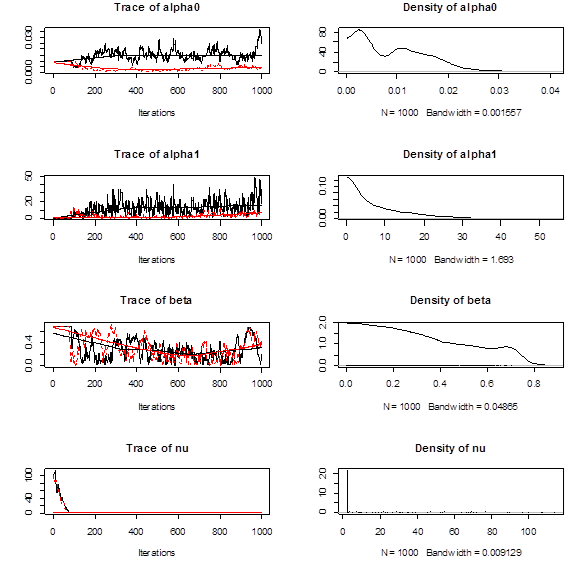
\includegraphics[width  = 8cm]{images/bayes-GARCH.png}
     \caption{bayesgarch轨迹图}
     \label{bayesgarch轨迹图}
     \end{figure}
    % \textcolor[rgb]{1.00,0.00,0.00}{todo:图片:bayesgarch轨迹图}
    \par
    设置参数向量$\alpha=(\alpha_0,\alpha_1 )$的先验分布中的初值为 0,$\Sigma_\alpha=diag(1000,1000)$,这里方差取1000是利用了扩散先验的思想,参数$\beta$的先验分布中的初值为 0,$\Sigma_\beta=1000$。为了确保收敛,我们模拟两条马氏链,每条迭代1000次,上图左边为迭代路径图,右边为后验分布的核密度估计。bayesGARCH模型参数估计结果如表(\ref{bayesGARCH模型参数估计结果})所示
        \begin{table}[H]
        \centering
        \caption{bayesGARCH模型参数估计结果}
        \label{bayesGARCH模型参数估计结果}
        \begin{tabular}{ccccc}
            \toprule
           Coefficient(s) & Mean  &  SD & Naive SE  &  Time-series SE\\
        \midrule
        alpha0 & 0.009656 &   0.007253  &  0.0003244  & 0.002069\\
        alpha1 & 9.363032 &   8.590657  &  0.3841858  & 2.216542\\
        beta  &  0.225654&    0.166916 &   0.0074647 &  0.032367\\
        nu & 2.034682 &   0.034131  &  0.0015264  & 0.014910\\
        \bottomrule
        \end{tabular}
        \end{table}
    % \textcolor[rgb]{1 0 0}{todo:表格:bayesGARCH模型参数估计结果}

    % \noindent 4、bayesGARCH模型参数估计结果
    % \textcolor[rgb]{1.00,0.00,0.00}{todo:表}
    % \noindent 5、IGARCH模型参数估计结果
    % \textcolor[rgb]{1.00,0.00,0.00}{todo:表}
    % \noindent 6、GARCHM模型参数估计结果
    % \textcolor[rgb]{1.00,0.00,0.00}{todo:表}
    % \noindent 7、eGARCH模型参数估计结果
    % \textcolor[rgb]{1.00,0.00,0.00}{todo:表}
    % \noindent 8、TGARCH模型参数估计结果
    % \textcolor[rgb]{1.00,0.00,0.00}{todo:表}
    % \noindent 9、nGARCH模型参数估计结果
    % \textcolor[rgb]{1.00,0.00,0.00}{todo:表}
    % \noindent 10、gjrGARCH模型参数估计结果
    % \textcolor[rgb]{1.00,0.00,0.00}{todo:表}
    % \noindent 11、apARCH模型参数估计结果
    % \textcolor[rgb]{1.00,0.00,0.00}{todo:表}
        \subsubsection{模型残差分析}
            \par
            在构建模型之前,我们对残差有一定的假设,我们假设残差为正态白噪声过程,因此,在建立模型之后,要对残差进行分析, 进行正态性检验、平稳性检验、相关性(独立性)检验和ARCH效应检验。利用Shapiro-Wilk.test进行正态性检验(不过不满足样本要求[50-80],后期修改),利用Box-Ljung.test进行独立性检验,利用LM.test进行ARCH效应检验。
            \paragraph{Shapiro-Wilk.test}
            Shapiro-Wilk.test的详细内容可以参考:数理统计P289或者梁小筠《正态性检验》P58。
            检验统计量为:
            \[T = W = \frac{{{{\left\{ {\sum\nolimits_{i = 1}^{[{\textstyle{n \over 2}}]} {{a_i}(W)[{x_{\left( {n + 1 - i} \right)}} - {x_{(i)}}]} } \right\}}^2}}}{{\sum\nolimits_{i = 1}^n {{{[{x_{(i)}} - \bar x]}^2}} }}\]
            其中:$\alpha_i$参考相关文献(梁小筠《正态性检验》P58)。
            \paragraph{Box-Ljung.test}
            独立性检验可以看作滞后期小于m期的序列值之间相互独立。
            原假设H0:
            \[{\rho _1} = {\rho _2} = \cdots = {\rho _m} = 0\]
            其中:$\rho_1$为滞后1期的自相关系数。
            备择假设H1:
            \[\exists i \in [1:q],{\rho _i} \ne 0\]
            一般情况下,我们只能得到样本的自相关函数值$̂\hat{\rho}_{i}$(即$\rho_i$的估计值),并且估计值一般不为0。 对$̂\hat{\rho}_{i}$有Bartlett 公式:如果$̂\hat{\rho}_{i}$在$r>M$时趋于0,则在$n$足够大的情况下,其方差为:
            \[D\left( {{{\hat \rho }_i}} \right) \approx \frac{1}{n}\sum\limits_{m =  - M}^M {\hat \rho _m^2} \]
            并且,$r>M$时,$̂\hat{\rho}_{i}$近似服从正态分布:
            \[{\hat \rho _i}\dot  \sim N\left( {0,\frac{1}{n}} \right)\]
            于是,有检验统计量Box-Pierce和Box- Ljung:
            \[{T_{BP}} = n\sum\limits_{i = 1}^m {\hat \rho _i^2}  \sim \chi \left( m \right)\]
            \[{T_{BL}} = n\left( {n + 2} \right)\sum\limits_{i = 1}^m {\frac{{\hat \rho _i^2}}{{n - k}}}  \sim \chi \left( m \right)\]
            \paragraph{LM.test}
            检验误差项$\varepsilon_t$是否服从ARCH(q)过程,也就是检验方程$\sigma_t^2=w+\Sigma_{i=1}^q{\alpha_i \varepsilon_{t-i}^2 }$ 中,所有回归系数$\alpha_i$ 是否同时为0。
            原假设H0:
            \[{\alpha _1} = {\alpha _2} = \cdots = {\alpha _m} = 0\]
            备择假设H1:
            \[\exists i \in [1:q],{\alpha _i} \ne 0\]
            构建LM检验统计量为:
            \[T = n\left(\frac{\partial L\left( \theta  \right)}{\partial \theta } \right)^{'}{I_\delta ^{-1}}{\left(\frac{\partial L\left( \theta  \right)}{\partial \theta } \right)}\]
            其中:$\theta=[\alpha_1,\alpha_2,…,\alpha_q],L(\theta)$为对数似然函数,$I_\delta^{-1}$为在似然函数最大时计算的信息阵倒数。计算公式如下:
            \[\frac{{\partial L\left( \theta  \right)}}{{\partial \delta }} = \frac{1}{2}\sum\limits_{t = 1}^n {\left\{ {\frac{{\varepsilon _t^2}}{{\sigma _t^2}} - 1} \right\}} \frac{{\partial \log \sigma _t^2}}{{\partial \delta }} - \sum\limits_{t = 1}^n {\frac{1}{{2\sigma _t^2}}} \frac{{\partial \varepsilon _t^2}}{{\partial \delta }}\]
            \begin{equation*}
            I_\delta  =  {{- \frac1n}E\left\{ {\frac{\partial ^2L\left( \theta  \right)}{\partial \delta \partial \delta ^{'}}}{\bigg|x_t} \right\} }
            \end{equation*}
            \begin{equation*}
            {\frac{\partial ^2L\left( \theta  \right)}{\partial \delta \partial \delta {'}}} = { - \frac12{\sum\limits_{t = 1}^n } {\frac{\varepsilon _t^2}{\sigma _t^2}}} {\frac{\partial \log \sigma _t^2}{\partial \delta }}{\frac{\partial \log \sigma _t^2}{\partial \delta '}}
            \end{equation*}
            信息矩阵的一致估计为:
            \begin{equation*}
            {\hat I_\delta } ={ \frac{1}{2n}\sum\limits_{t = 1}^n }{\frac{z_t\left( \theta  \right)z_t\left( \theta  \right)'}{{\left( \sigma _t^2 \right)}^2}}
            \end{equation*}
        \subsubsection{模型评价6个指标}
            \par
            前面,我们对单一的FB收益率序列建立了诸多的模型,那么,接下来的问题很自然就是如何来评价这些模型,这是一个很重要的问题,这将指导我们对FB序列建立最适合的模型,从而进行最好的估计与预测。在线性回归中,我们利用$R^2$来评价模型,虽然我们也可以用其来评价模型,但此并非常用准则。下面,我们来构建模型的评价指标:
            \par
            1、AIC信息准则:
            AIC(Akaika information criterion)信息准则由日本统计学家Akaika于1973年提出,该准则不仅考虑了模型对数据的拟合程度,还考虑了模型参数的个数。AIC的一般形式为:AIC = - 2ln(模型最大似然度) + 2(模型独立参数个数)
            \[
            AIC = n\left[ {\log \left( {\frac{{RSS}}{n}} \right) + 1 + \log (2\pi )} \right] + 2(p + 1)
            \]
            其中:RSS是拟合残差平方和,$p$是选入模型的参数$(p=p+q=1+1)$,$n$为样本量。
            \par
            2、BIC信息准则:
            由于AIC方法不能给出相容估计(当样本量$n$趋近于无穷时,采用AIC方法定出的模型阶数不能依概率收敛到真值,通常比真值要高),为此,Akaike和E.J.Haman于1979年又提出了BIC准则,BIC的一般形式为:
            BIC = - 2ln(模型最大似然度) + 2(模型独立参数个数)
            \[
            BIC = n\left[ {\log \left( {\frac{{RSS}}{n}} \right) + 1 + \log (2\pi )} \right] + (p + 1)\log (n)
            \]
            \par
            3、模型残差结果:
            汇总各模型残差的随机性检验(LBtest)、ARCH检验(LMtest)和正态性检验。
            \par
            4、6个误差指标:
            在2002年,Buhlmann和McNeil定义了以下6个误差指标来评价模型:平均平方误差(MSE1、MSE2)、平均绝对误差(MAE1、MAE2)、高斯准极大似然损失函数误差(QLIKE)及对数损失函数误差($R^2LN $)。
            \begin{equation*}
            \centering
            \left\{\begin{lgathered}
            MSE1 = \frac{1}{n}\sum\limits_{t = 1}^n {{{\left( {{{\hat \sigma }_t} - {\sigma _t}} \right)}^2}} \\
            MSE2 = \frac{1}{n}\sum\limits_{t = 1}^n {{{\left( {\hat \sigma _t^2 - \sigma _t^2} \right)}^2}} \\
            MAE1 = \frac{1}{n}\sum\limits_{t = 1}^n {\left| {{{\hat \sigma }_t} - {\sigma _t}} \right|} \\
            MAE2 = \frac{1}{n}\sum\limits_{t = 1}^n {\left| {\hat \sigma _t^2 - \sigma _t^2} \right|} \\
            QLIKE = \frac{1}{n}\sum\limits_{t = 1}^n {\left( {\ln \hat \sigma _t^2 + {{\sigma _t^2} \mathord{\left/
             {\vphantom {{\sigma _t^2} {\hat \sigma _t^2}}} \right.
             \kern-\nulldelimiterspace} {\hat \sigma _t^2}}} \right)} \\
            {R^2}LN = \frac{1}{n}\sum\limits_{t = 1}^n {{{\left( {\ln {{\sigma _t^2} \mathord{\left/
             {\vphantom {{\sigma _t^2} {\hat \sigma _t^2}}} \right.
             \kern-\nulldelimiterspace} {\hat \sigma _t^2}}} \right)}^2}}
             \end{lgathered} \right.
             \end{equation*}
            其中,$n$为样本大小,$\sigma_t$为误差项$\varepsilon_t$的标准差,$\hat{\sigma}_t$为其估计值,$\sigma_t^2$ 为条件方差(即误差项$\varepsilon_t$的条件异方差)。MSE1、MSE 2、MAE1、MAE2越小表示预测精度越高,QLIKE 和$R^2LN$ 越大表示预测精度越高。
            \par
            值得一提的是,在ruGARCH包中,编者将AIC等信息编写为如下形式:
            \begin{equation*}
            \centering
            \left\{\begin{lgathered}
            AIC = \frac{{ - 2LLH}}{N} + \frac{{2m}}{N}\\
            BIC = \frac{{ - 2LLH}}{N} + \frac{{m{{\log }_e}\left( N \right)}}{N}\\
            HQIC = \frac{{ - 2LLH}}{N} + \frac{{2m{{\log }_e}\left( {{{\log }_e}\left( N \right)} \right)}}{N}\\
            SIC = \frac{{ - 2LLH}}{N} + {\log _e}\left( {\frac{{N + 2m}}{N}} \right)
             \end{lgathered} \right.
             \end{equation*}
    \subsection{GARCH族模型结果分析}
        \par
        根据前面的bayesGARCH模型的结果
        % (bayesGARCH模型的Stationarity.test和Halfwidth.test)
        可以看到,bayesGARCH模型的估计结果并不令人满意。Gelman和Rubin于1992年提出的方差比法:如果$\hat{R}>1$,说明链收敛不好;如果$\hat{R}=1$,说明链达到静止状态。而上面bayesGARCH模型的方差大于1,说明模型不理想。改进的方向有:1、调整初始值2、增加迭代次数等。
        % \textcolor[rgb]{1.00,0.00,0.00}{todo:表格:bayesGARCH模型的Stationarity.test和Halfwidth.test}
        总之,bayesGARCH建模失败了,这个模型我们以后再讨论。下面,我们分析一下其他的模型:
        \begin{enumerate}
        \item 就AIC和BIC信息而言,AIC等准则越小越好(但这仅就同模型而言,不同模型之间还未考虑),而girGARCH模型的AIC是最小的,IGARCH模型仅次之,并且两个模型之间有一定的联系;就BIC而言apARCH模型是最优的,gjrGARCH模型仅次之。
        \item 就残差正态性检验而言,由于我们在上述建模过程中,均假设残差服从正态分布,因此,有必要进行正态性检验,在SWtest下,所有模型均在0.05的显著水平下拒绝正态原假设。不过这里使用的检验方法有一些问题,有待后续研究(可以用不同的正态性检验方法进行比较)。
        \item 就残差的独立性而言,仅有ARMA模型没有拒绝原假设(原假设为独立随机),其他模型均在0.05的显著水平下拒绝原假设。
        \item 残差的ARCH效应检验,仅有ARMA和GARCHM模型没有拒绝原假设(原假设为无GARCH效应),其他模型均在0.05的显著水平下拒绝原假设。
        \item 就6个拟合指标而言,ARMA模型在MSE1、MSE2、MAE2和QLIKE指标下均优于其他模型,而apARCH模型则占据了MAE1和R2LE指标的榜首。
        \end{enumerate}
        \par
        综上而言,ARMA模型较为适合FB收益率,其次是apARCH和gjrGARCH(IGARCH)。一种更为有利的比较方法是在每个指标下,将模型排名,然后汇总最终的排名结果(如取均值等方法)。
            \begin{figure}[H]
            \centering
            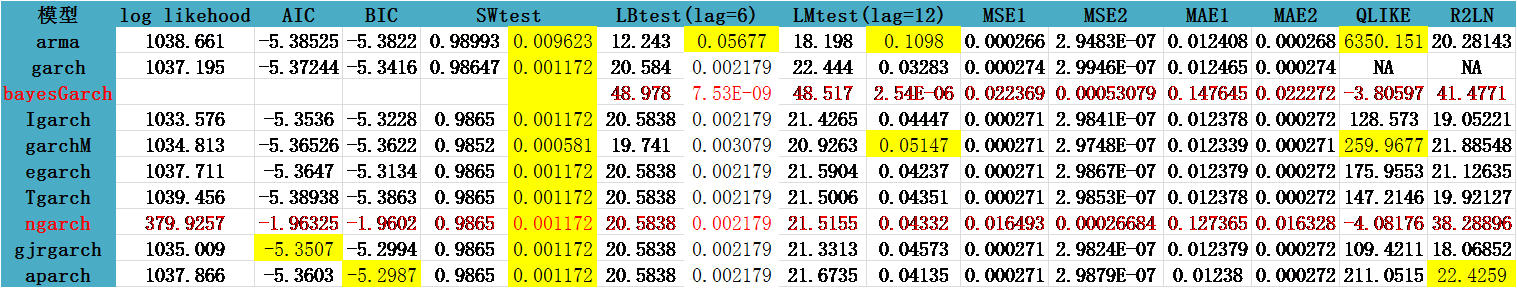
\includegraphics[angle=90,width=4cm]{images/model_result_summary.jpg}
            \caption{模型结果汇总表}
            \label{模型结果汇总表}
            \end{figure}
        % \textcolor[rgb]{1.00,0.00,0.00}{todo:图片;模型结果汇总表}
    \subsection{程序}
        由于各个模型的建模基本相似,这里我们仅给出部分模型的程序。以IGARCH模型为例,IGARCH模型的建模程序如下
        \begin{lstlisting}[language = R]
        ############# rugarch package 介绍##
        #http://unstarched.net/r/rugarch/  原始路径
        #http://herbert12.blog.163.com/blog/static/304782320120184118846/
        #http://www.biostatistic.net/thread-78659-1-1.html  翻译
        .libPaths("D:/Program Files/R/R-3.1.3/library")
        install.packages("rugarch", lib = "D:/Program Files/R/R-3.1.3/library")
        library(parallel)
        #install.packages("truncnorm", lib = "D:/Program Files/R/R-3.1.3/library")
        install.packages("misc3d", lib = "D:/Program Files/R/R-3.1.3/library")
        install.packages("rgl", lib = "D:/Program Files/R/R-3.1.3/library")
        library(rugarch)
        #该模型由三个部分构成,均值方程对应式(1),分布假设对应(2),方差方程对应式(3),
        # 对三个部分进行适当的变形后可以形成
        # egarch模型,egarch-ged模型,egarch-t模型,Igarch模型,garch-m模型和Qgarch模型等
        # 因此,设定模型形式就是分别设定均值方程、方差方程和分布。
        # spec=ugarchspec(variance.model = list(model = "sGARCH", garchOrder = c(1, 1),
        #                                       submodel = NULL,
        #                                       external.regressors = NULL,
        #                                       variance.targeting = FALSE),
        #                 mean.model = list(armaOrder = c(1, 1),
        #                                   include.mean = TRUE,
        #                                   archm = FALSE,
        #                                   archpow = 1,
        #                                   arfima = FALSE,
        #                                   external.regressors = NULL,
        #                                   archex = FALSE),
        #                 distribution.model = "norm")
        # ugarchfit(spec,
        #           data,
        #           out.sample = 0,
        #           solver = "solnp",
        #           solver.control = list(),
        #           fit.control = list(stationarity = 1, fixed.se = 0, scale = 0, rec.init = 'all'),
        #           numderiv.control = list(grad.eps=1e-4, grad.d=0.0001,
        #                                   grad.zero.tol = sqrt(.Machine$double.eps/7e-7),
        #                                   hess.eps = 1e-4,
        #                                   hess.d = 0.1,
        #                                   hess.zero.tol = sqrt(.Machine$double.eps/7e-7),
        #                                   r=4, v=2))
        # 通过plot(myfit)可以对模型结果进行图形诊断:
        # plot(myfit)  # Make a plot selection (or 0 to exit):  1:   Series with 2 Conditional SD
        ###################exapmle for rugarch package
        variance.model <- list(model = "eGARCH", garchOrder = c(2, 3))
        # # model Valid models (currently implemented) are “sGARCH”, “fGARCH”, “eGARCH”, “gjrGARCH”, “apARCH” and “iGARCH” and “csGARCH”.
        # # garchOrder The ARCH (q) and GARCH (p) orders.
        # # submodel If the model is “fGARCH”, valid submodels are “GARCH”, “TGARCH”, “AVGARCH”, “NGARCH”, “NAGARCH”, “APARCH”,“GJRGARCH” and “ALLGARCH”.
        mean.model <- list(armaOrder = c(0, 0), include.mean = T, archm = F)
        spec <- ugarchspec(variance.model = variance.model,
                           mean.model = mean.model,
                           distribution.model = "norm")
        fit <- ugarchfit(spec = spec,
                          data = xt,
                         out.sample = 0,
                         solver = "solnp",
                          solver.control = list(trace = 0))
        #
        #model four:Igarch#######################################################
        ##方法1:######
        source("Igarch.R")#Igarch.R在下面给出
        model4.Igarch <- Igarch(as.vector(xt), include.mean = T)
        smodel4.Igarch$model.information
        ##方法2:use rugarch package##
        variance.model <- list(model = "iGARCH", garchOrder = c(1, 1))
        mean.model <- list(armaOrder = c(0, 0), include.mean = T, archm = F)
        distribution.model <- "norm"
        spec.igarch <- ugarchspec(variance.model = variance.model,
                                   mean.model = mean.model,
                                   distribution.model = distribution.model)
        model4.Igarch.rugarch <- ugarchfit(spec = spec.igarch,
                                           data = xt,
                                           out.sample = 0,
                                           solver = "solnp",
                                           solver.control = list(trace = 0))
        #模型信息
        model4.Igarch.rugarch
        #计算模型6个指标
        re.IgarchModel.rugarch <- model4.Igarch.rugarch@fit$residuals  #residuals(model4.Igarch.rugarch)
        fit.IgarchModel.rugarch <- model4.Igarch.rugarch@fit$fitted.values  #fitted(model4.Igarch.rugarch)
        if(length(xt) == length(fit.IgarchModel.rugarch))
          a <- rbind(a, criterion(fit.IgarchModel.rugarch, xt))
        #模型残差的分析
        shapiro.test(re.IgarchModel.rugarch)#正态性检验
        Box.test(re.IgarchModel.rugarch,
                 lag = ceiling(log(length(re.IgarchModel.rugarch))),
                 type = "Ljung-Box")
        ArchTest(re.IgarchModel.rugarch, lag = 12)
        \end{lstlisting}
        \par
        上面用到的Igarch函数如下
        \begin{lstlisting}[language = R]
        "Igarch" <- function(rtn,include.mean=F,volcnt=F){
        # Estimation of a Gaussian IGARCH(1,1) model.
        # rtn: return series
        # include.mean: flag for the constant in the mean equation.
        # volcnt: flag for the constant term of the volatility equation.
        #### default is the RiskMetrics model
        #
        Idata <<- rtn
        Flag <<- c(include.mean,volcnt)
        #
        Mean=mean(Idata); Var = var(Idata); S = 1e-6
        if((volcnt)&&(include.mean)){
        params=c(mu = Mean,omega=0.1*Var,beta=0.85)
        lowerBounds = c(mu = -10*abs(Mean), omega= S^2, beta= S)
        upperBounds = c(mu = 10*abs(Mean), omega = 100*Var, beta = 1-S)
        }
        if((volcnt)&&(!include.mean)){
        params=c(omega=0.1*Var, beta=0.85)
        lowerBounds=c(omega=S^2,beta=S)
        upperBounds=c(omega=100*Var,beta=1-S)
        }
        #
        if((!volcnt)&&(include.mean)){
        params=c(mu = Mean, beta= 0.8)
        lowerBounds = c(mu = -10*abs(Mean), beta= S)
        upperBounds = c(mu = 10*abs(Mean), beta = 1-S)
        }
        if((!volcnt)&&(!include.mean)){
        params=c(beta=0.85)
        lowerBounds=c(beta=S)
        upperBounds=c(beta=1-S)
        }
        # Step 3: set conditional distribution function:
        igarchDist = function(z,hh){dnorm(x = z/hh)/hh}
        # Step 4: Compose log-likelihood function:
        igarchLLH = function(parm){
        include.mean=Flag[1]
        volcnt=Flag[2]
        mu=0; omega = 0
        if((include.mean)&&(volcnt)){
        my=parm[1]; omega=parm[2]; beta=parm[3]}
        if((!include.mean)&&(volcnt)){
        omega=parm[1];beta=parm[2]}
        if((!include.mean)&&(!volcnt))beta=parm[1]
        if((include.mean)&&(!volcnt)){mu=parm[1]; beta=parm[2]}
        #
        z = (Idata - mu); Meanz = mean(z^2)
        e= omega + (1-beta)* c(Meanz, z[-length(Idata)]^2)
        h = filter(e, beta, "r", init=Meanz)
        hh = sqrt(abs(h))
        llh = -sum(log(igarchDist(z, hh)))
        llh
        }
        # Step 5: Estimate Parameters and Compute Numerically Hessian:
        fit = nlminb(start = params, objective = igarchLLH,
        lower = lowerBounds, upper = upperBounds)
        ##lower = lowerBounds, upper = upperBounds, control = list(trace=3))
        epsilon = 0.0001 * fit$par
        cat("Estimates: ",fit$par,"\n")
        npar=length(params)
        Hessian = matrix(0, ncol = npar, nrow = npar)
        for (i in 1:npar) {
        for (j in 1:npar) {
        x1 = x2 = x3 = x4  = fit$par
        x1[i] = x1[i] + epsilon[i]; x1[j] = x1[j] + epsilon[j]
        x2[i] = x2[i] + epsilon[i]; x2[j] = x2[j] - epsilon[j]
        x3[i] = x3[i] - epsilon[i]; x3[j] = x3[j] + epsilon[j]
        x4[i] = x4[i] - epsilon[i]; x4[j] = x4[j] - epsilon[j]
        Hessian[i, j] = (igarchLLH(x1)-igarchLLH(x2)-igarchLLH(x3)+igarchLLH(x4))/
        (4*epsilon[i]*epsilon[j])
        }
        }
        cat("Maximized log-likehood: ",igarchLLH(fit$par),"\n")
        # Step 6: Create and Print Summary Report:
        se.coef = sqrt(diag(solve(Hessian)))
        tval = fit$par/se.coef
        matcoef = cbind(fit$par, se.coef, tval, 2*(1-pnorm(abs(tval))))
        dimnames(matcoef) = list(names(tval), c(" Estimate",
        " Std. Error", " t value", "Pr(>|t|)"))
        cat("\nCoefficient(s):\n")
        printCoefmat(matcoef, digits = 6, signif.stars = TRUE)

        if((include.mean)&&(volcnt)){
        mu=fit$par[1]; omega=fit$par[2]; beta = fit$par[3]
        }
        if((include.mean)&&(!volcnt)){
        mu = fit$par[1]; beta = fit$par[2]; omega = 0
        }
        if((!include.mean)&&(volcnt)){
        mu=0; omega=fit$par[1]; beta=fit$par[2]
        }
        if((!include.mean)&&(!volcnt)){
        mu=0; omega=0; beta=fit$par[1]
        }
        z=Idata-mu; Mz = mean(z^2)
        e= omega + (1-beta)*c(Mz,z[-length(z)]^2)
        h = filter(e,beta,"r",init=Mz)
        vol = sqrt(abs(h))

        Igarch <- list(par=fit$par,
                       volatility = vol,
                       model.information = matcoef,
                       model.loglikehood = igarchLLH(fit$par))
        }
        \end{lstlisting}

\section{应用}
    \par
    对组合投资和期权定价的研究一直是金融领域的热点问题。随经济的发展和网络时代的到来,投资渐渐成为人们的生活必需品,投资相对于存款而言,最大区别在于,投资的收益是与风险相伴的,而人们在对多种投资对象(股票)进行投资时,往往期望在一定投资期内,投资风险最小下,投资(组合)带来的利益最大。
    % 金融数学又称为分析金融学,是计算机、数学和金融相结合的学科,主要运用随机分析、最优化方法、最优控制、组合分析等数学方法来探讨金融衍生品的定价、组合投资和风险控制等问题。
    \par
    1900年Louis Bachelier在“The Theory of Speulation”中首次提出使用Brown运动来分析股票价格变换,但可惜的是,这种方法直到后来才被人们所接受。现代金融学发生过两场历史性革命:第一次革命是由1990年诺贝尔经济学奖得主Markowitz.H引起的,1952年Markowitz在其博士论文中创造性的建立了均值-方差组合投资模型来定量计量组合的风险和收益后,数理工具在金融领域开始大放异彩,它突破了传统金融,渐渐在金融工程中占据主导地位。第二次革命是由1997年诺贝尔经济学奖得主Scholes等引起的,Black.F和Scholes.M运用随机微分方程对股票价格进行模拟,并提出了著名的欧式期权定价公式:Black - Scholes定价公式。
    \par
    Markowitz的组合投资策略是基于均值 - 方差的,他用股票收益率的均值作为股票收益的度量,用收益率的方差作为风险的度量,投资的最终目标是使投资的收益最大风险最小。Markowitz用收益率的方差来定量计算投资风险的方法并非没有缺陷,方差只描述了收益率偏离期望的程度,没有反应偏离方向,但人们通常关心负偏离带来的损失,方差也不能反应证券组合的损失由多大。随着风险的不同度量方法的进化,均值-方差模型后续又进化为:均值 - 半方差、均值 - 绝对差、均值 - VaR、均值 - CVaR等,然而,在传统的均值 - 方差模型族中,收益率的均值和方差是不随时间变化的,这与实际情况并不相符,人们对收益率的认识已经从正态白噪声中脱离出来,已经有一系列描述收益率情况的模型,比如ARCH族、SV族等。并且,对于股票收益率的建模,不仅仅局限于时间序列模型,还有前面介绍的随机微分方程等可以使用。
    \subsection{收益率模型}
        \par
        由于在下面的组合投资和期权定价问题中,收益率都占据着非常重要的地位,因此,我们先建立收益率模型。由于不同市场的基数不同,我们设收益率为:
        \begin{align*}
        x_t = \ln \frac{P_t}{P_{t-1}} = \ln P_t -\ln P_{t-1}
        \end{align*}
        其中:$P_t$为$t$时刻的股票价格,我们可以用前面介绍的SDE(随机微分方程)进行模拟,这里,我们直接用GARCH模型族对其进行模拟。在平稳的前提下,我们对 $\{x_t\}$建立GARCH模型。
        % ,GARCH模型如下
        % \begin{align*}
        % \left\{
        % \begin{aligned}
        % & x_t = c+\sum_{i=1}^r\varphi_i r_{t-i}+\sum_{i=1}^m\theta_i\varepsilon_{t-i}\\
        % & \varepsilon_t = \sigma_t v_t\\
        % & \sigma_t^2 = d+\sum_{i=1}^p\beta_{t-i}^2+\sum_{i=1}^q\alpha_i\varepsilon_{t-i}^2\\
        % & v_t\sim N(0,1)\quad iid
        % \end{aligned}
        % \right.
        % \end{align*}
        % 其中:$x_t$为收益率序列,$\varepsilon_t$为具有ARCH效应的白噪声,$\sigma_t^2$为方差序列,$\phi,\theta,\alpha,\beta$为系数。ARCH效应是对残差的波动密集性的描述,本质上是对残差序列的平方$\{\varepsilon_t^2\}$建立AR模型。

    \subsection{风险度量:条件风险价值CVaR}
        \par
        在上面的收益率模型中,我们已经计算了收益率的均值和方差,然而,方差并不能很好的度量风险。方差只描述了收益率偏离期望的程度,没有反应偏离方向,但人们通常关心负偏离带来的损失,方差也不能反应证券组合的损失由多大,因此,我们采用基于风险价值VaR的条件风险价值来度量风险。
        \begin{definition}[风险价值VaR]
        某项金融资产(例如股票和股票的组合)在一定时期内,在一定置信水平下,可能的最大损失
        \begin{align*}
        P\{x_t < VaR_t\} = \alpha
        \end{align*}
        其中:$x_t$为$t$时刻的收益率,$\alpha$为显著性水平(百分位数),$1-\alpha$为置信水平。
        \end{definition}
        \par
        用VaR作为风险的度量有一定的缺陷,他没有考虑尾部风险,即损失超过VaR的风险,VaR不满足其次可加性,为此,我们引入具有次其次可加特点的条件风险价值CVaR来度量风险。CVaR是在一定置信水平下,发生损失超过VaR时的平均损失。计算公式如下
        \begin{align*}
        CVaR_t = -\mathbb{E}(x_t|x_t \leqslant -VaR_t ) = \frac{\int_{-\infty}^{VaR_t}zf(z)\mathrm{d}z}{1-\alpha}
        \end{align*}
        其中:$f(\cdot)$为收益率的概率密度函数。
        \par
        计算VaR和CVaR的方法有许多,如历史模拟法、分析法、Monte Carlo模拟法、极值法等。下面的计算中,我们主要利用正态法进行求解。
        \par
        (1)CF展开法求VaR和CVaR:Cornish - Fisher展开式将标准化后的收益率的百分位数 $\alpha$近似表示为
        \begin{align*}
        q = c(\alpha)+\frac{1}{6} [c(\alpha)^2-1]s_t+\frac{1}{24}[c(\alpha)^3-3c(\alpha)][k_t-3]-\frac{1}{36}[c(\alpha)^3-5c(\alpha)]s_t^2
        \end{align*}
        其中:$c(\alpha)$为标准正态分布的$\alpha$百分位数,$s_t$为标准收益的偏度,$k_t$为标准收益的峰度。所以,我们可以计算CVaR的近似展开式,收益率$x_t$的百分位数$\alpha$为
        \begin{align*}
        VaR_t = u_t + \sigma_tq
        \end{align*}
        CVaR为
        \begin{align*}
        CVaR_t = -\sigma_t \left( M_1+\frac{1}{6}(M_2-1)s_t+\frac{1}{24}(M_3-3M_1)(k_t-3-\frac{1}{36} \right) (2M_3-5M_1)s_t^2
        \end{align*}
        其中:$M_i = \frac{1}{\alpha_i} = \int_{-\infty}^{c(\alpha)}x^if(x)\mathrm{d}x,i=1,2,3$,$f(\cdot)$为标准正态分布的密度函数。
        \par
        (2)基于正态分布的 VaR 和CVaR:设各时点$t$上收益率$r$服从具有时变方差的条件正态分布,所以有
        \begin{align*}
        x_t|I_{t-1} \sim N(\mu_t,\sigma_t^2)
        \end{align*}
        所以正态分布下的VaR 和CVaR为
        \begin{align*}
        & VaR_t = -\mu_t+c(1-\alpha)\sigma_t\\
        & CVaR_t = -\mu_t-\sigma_tf(c(1-\alpha))/(1-\alpha)
        \end{align*}
    \subsection{组合投资E-CVaR模型}
        \par
        组合投资即为用有限的资金来投资不同的股票。当然,在投资后的一定时期,我们将会获得投资的回报,虽然有时回报可能是负值,我们自然很希望我们的投资选择是最好的:风险最小,收益最大。我们将股票数目确定,规定必须要投资也只能投资某些股票,我们用每个股票的收益率均值E作为收益的度量,用每个股票收益率的条件风险价值CVaR作为风险的度量,我们可以依据每个股票的历史收益率序列来计算均值E和条件风险价值CVaR,我们希望在我们投资过后,组合投资的收益最大,风险最小,这就使得我们需要确定我们的投资权重,也就是将固定资产的多少用于投资某个股票。当然,区别于传统的组合投资,组合投资E-CVaR的投资时间也是非常关键的,因为,我们的收益率均值E和收益率条件风险价值CVaR都是和时间有关的。这说明,在收益最大、风险最小这个多目标下,我们的投资权重和投资时间将是决定性变量(所求)。下面,我们来建立与时间有关的E-CVaR模型。
        \par
        设有$n$个投资对象($n$个股票),每个股票记为$i$,$t$时刻股票$i$的价格记为$P_t^i$,$t$时刻股票$i$的收益率序列为$x_t^i$,股票$i$的投资权重为$w_i$,投资时间限制为$T$时间内,则E-CVaR模型为
        \begin{align*}
        & \min\ \sum_{i=1}^n CVaR_t^i \cdot w_i\\
        & \max\ \sum_{i=1}^n \mathbb{E}(x_t^i)\cdot w_i\\
        & s.t.\left\{
        \begin{aligned}
        & \sum_{i=1}^n w_i =1\\
        & 0 \leqslant w_i \leqslant 1\\
        & 0 \leqslant t \leqslant T\\
        & i=1,2,\dots,n
        \end{aligned}
        \right.
        \end{align*}
    \subsection{组合投资的数值模拟}
        \par
        \textbf{数据}:我们通过MATLAB链接Yahoo财经网,从而获取投资对象的信息(股票的历史价格),选取IT行业的主要企业进行投资,他们分别是:'AAPL'、'GOOG'、'FB'、'AMZN'、'PCLN'、'BIDU'、'YHOO'、'JD'、'NFLX'、'LNKD'、'TWTR'和'TRIP'。经过简单的处理后,排除'GOOG', 'JD'和'TWTR'3支股票,选取剩余9支股票的截至到12/01/2015的889个日期股票价格数据作为组合投资对象。
        \par
        \textbf{目标}:我们首先对每只股票价格进行收益率处理,然后构建每只股票的收益率序列模型,并计算每支股票的风险价值和条件风险价值序列,计算各个时点$t$的E - VaR、E - CVaR模型的有效前沿;最终计算最优的组合权重$w_i$。
        \par
        对9支股票收益率序列建立GARCH模型。其中,均值模型建立ARMA模型,方差模型建立GARCH模型,收益率模型的部分信息如表(\ref{9个收益率模型的信息})所示。在表(\ref{9个收益率模型的信息})中,有收益率序列的平稳性检验、均值、均值模型ARMA的阶数$r$和$m$、均值模型后的残差ARCH效应检验、方差模型GARCH的阶数$p$和$q$、方差模型的模型信息AIC和BIC以及方差模型后的残差ARCH效应检验。
        \begin{table}[H]
        \footnotesize
        \caption{9个收益率模型的信息}
        \label{9个收益率模型的信息}
        \centering
        \begin{tabular}{c|ccccccccc}
            \toprule
            收益率 &$r1$ & $r2$&  $r3$ & $r4$ & $r5$ & $r6$ & $r7$ & $r8$ & $r9$\\
            \midrule
            平稳性 &平稳 & 平稳 & 平稳 & 平稳 & 平稳 & 平稳 & 平稳 & 平稳 & 平稳\\
            均值 & 0.0014  &-0.0012& -0.0007 &-0.0012& -0.0006& -0.0009& -0.0009 &-0.0009& -0.0013\\
            $r$ &  6  & 1  & 1  & 0  & 1  & 1 &  0  & 2  & 0\\
            $m$ &  4  & 1  & 1  & 1  & 0   &3 &  1  & 5  & 1\\
            异方差 &TRUE  &  FALSE  & FALSE &  FALSE &  FALSE  & FALSE  & FALSE  & FALSE &  FALSE\\
            $p$ &  1 &  0  & 2 &  0  & 0 &  1  & 0  & 1 &  0\\
            $q$  & 1  & 0  & 1  & 0  & 0 &  1  & 0  & 1  & 0\\
            $aic$& -4714.30 &   -3924.17 &   -4427.40 &   -4417.54  &  -3993.14&    -4598.48 &   -3191.88   & -3700.50 &   -3874.82\\
            $bic$ &-4699.93   & -3919.38   & -4408.23 &   -4412.75  &  -3988.35  &  -4584.11   & -3187.09   & -3686.12  &  -3870.03\\
            异方差 &FALSE  & FALSE  & TRUE  &  FALSE  & FALSE  & TRUE  &  FALSE  & TRUE &   FALSE\\
            \bottomrule
        \end{tabular}
        \end{table}
        下面,详细给出收益率序列$r6$(AMZN)的模型以及利用模型生成的收益率序列$r6$(AMZN)的均值和方差。收益率序列$r6$(AMZN)的模型为
        \begin{align*}
        \left\{
        \begin{aligned}
        & x_t = -0.0009+0.6355r_{t-1}+\varepsilon_t-0.6312\varepsilon_{t-1}-0.001846\varepsilon_{t-2}-0.09839\varepsilon_{t-3}\\
        & \sigma_t^2 = 0.823793\sigma_{t-1}^2+0.1127\varepsilon_{t-1}^2
        \end{aligned}
        \right.
        \end{align*}
        收益率序列图和收益率序列均值模拟图,方差模拟图如图(\ref{r6均值方差模拟图})所示。
        \begin{figure}[H]
        \centering
        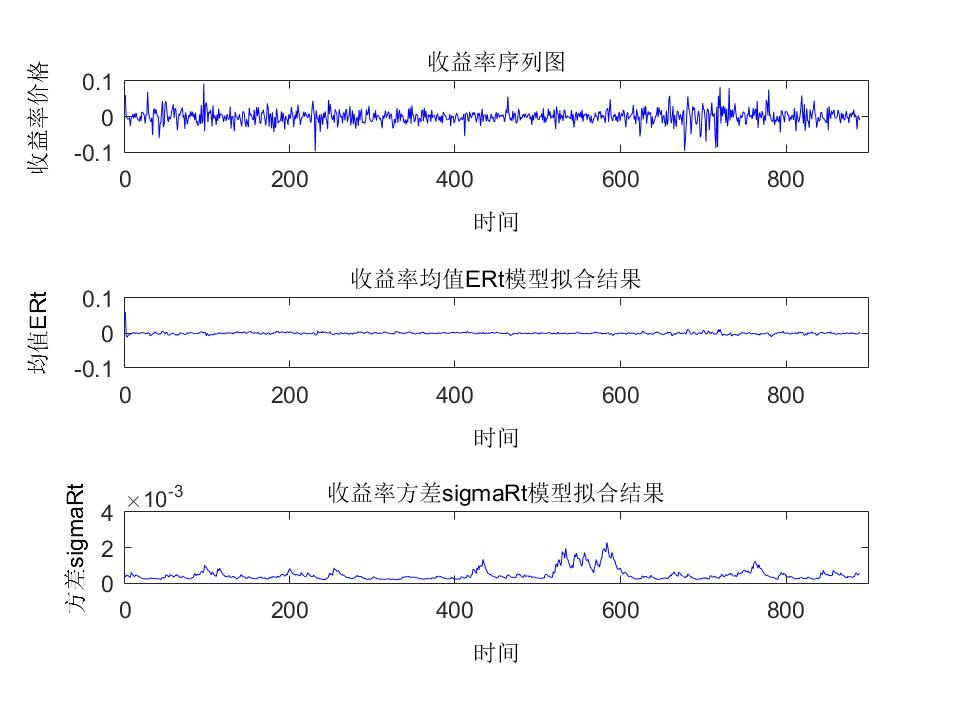
\includegraphics[width= 8cm]{images/r6_mu_sigma.jpg}
        \caption{$r6$均值方差模拟图}
        \label{r6均值方差模拟图}
        \end{figure}
        \par
        利用正态分布下的VaR 和CVaR计算公式
        \begin{align*}
        & VaR_t = -\mu_t + c(1-\alpha)\sigma_t\\
        & CVaR_t = -\mu_t-\sigma_tf(c(1-\alpha))/(1-\alpha)
        \end{align*}
        得到的9支股票收益率序列的条件风险价值$CVaR_t$ 如表(\ref{9支股票收益率序列的条件风险价值})\footnote{注:()表示取负值。例如:(0.0101)表示-0.0101}所示
        \begin{table}[H]
        \footnotesize
        \caption{9支股票收益率序列的条件风险价值}
        \label{9支股票收益率序列的条件风险价值}
        \centering
        \begin{tabular}{lllllllll}
            \toprule
        AAPL      &   FB       &  AMZN   & PCLN     & BIDU     & YHOO     & NFLX     & LNKD     & TPIP\\
                    \midrule
        0.0109    &   0.0108   &  0.0028 & 0.0097   & (0.0078) & (0.0597) & 0.0028   & (0.0462) & (0.0075)\\
        (0.0101)  &   (0.0107) &  0.0025 & (0.0005) & (0.0008) & 0.0041   & (0.0010) & (0.0039) & (0.0007)\\
        (0.0159)  &   0.0082   &  0.0023 & (0.0010) & (0.0006) & 0.0109   & (0.0000) & 0.0050   & (0.0008)\\
        (0.0033)  &   (0.0092) &  0.0029 & (0.0008) & (0.0007) & 0.0068   & (0.0029) & 0.0234   & (0.0007)\\
        0.0068    &   0.0071   &  0.0025 & (0.0003) & (0.0007) & 0.0043   & (0.0006) & 0.0226   &  0.0002 \\
            \bottomrule
        \end{tabular}
        \end{table}
        \par
        我们选取$t$时刻进行研究,观察9支股票的不同组合投资模型下的有效前沿(不许买空)。其中,不同的组合投资模型包括:CVaR - E,VaR - E,sigma - E,分别是利用条件风险价值、风险价值、方差来度量风险。t时刻的9支股票的均值、方差、风险价值、条件风险价值如表(\ref{(t=889)时刻的9支股票的均值、方差、风险价值、条件风险价值})所示
        \begin{table}[H]
        \footnotesize
        \caption{$t=889$时刻的9支股票的均值、方差、风险价值、条件风险价值}
        \label{(t=889)时刻的9支股票的均值、方差、风险价值、条件风险价值}
        \centering
        \begin{tabular}{l|lllllllll}
            \toprule
        股票 & AAPL &   FB & AMZN  &  PCLN  &  BIDU  &  YHOO  &  NFLX  &  LNKD  &  TPIP\\
            \midrule
        E    &2.74E-04  &-2.45E-03& -5.93E-04 &-1.58E-03& -7.91E-04& 1.93E-03 & 3.43E-03 & 3.56E-03 &-2.75E-03\\
        sigma&3.57E-04  &7.07E-04 & 3.77E-04  &4.06E-04 & 6.54E-04 & 3.53E-04 & 1.61E-03 & 1.44E-03 & 7.48E-04\\
        VaR  &4.50E-02  &6.32E-02 & 4.51E-02  &4.72E-02 & 5.97E-02 & 4.09E-02 & 8.91E-02 & 8.38E-02 & 6.50E-02\\
        CVaR &6.04E-04  &5.78E-04 & -6.25E-04 &-1.92E-04& -4.65E-04& -3.30E-03& -5.37E-03& -5.52E-03& 6.80E-04\\
            \bottomrule
        \end{tabular}
        \end{table}
        \par
        有效组合是指在同样风险水平下具有最高收益的组合,不同的收益及不同收益对应的最小风险记为有效前沿。$t (t=889)$时刻9支股票的不同模型的有效前沿如图(\ref{各种组合模型的有效前沿})所示,每一个收益ER都会对应一个最小的风险,在大多数情况下,我们更加关心收益为正(ER>0)时的风险。
        \begin{figure}[H]
        \centering
        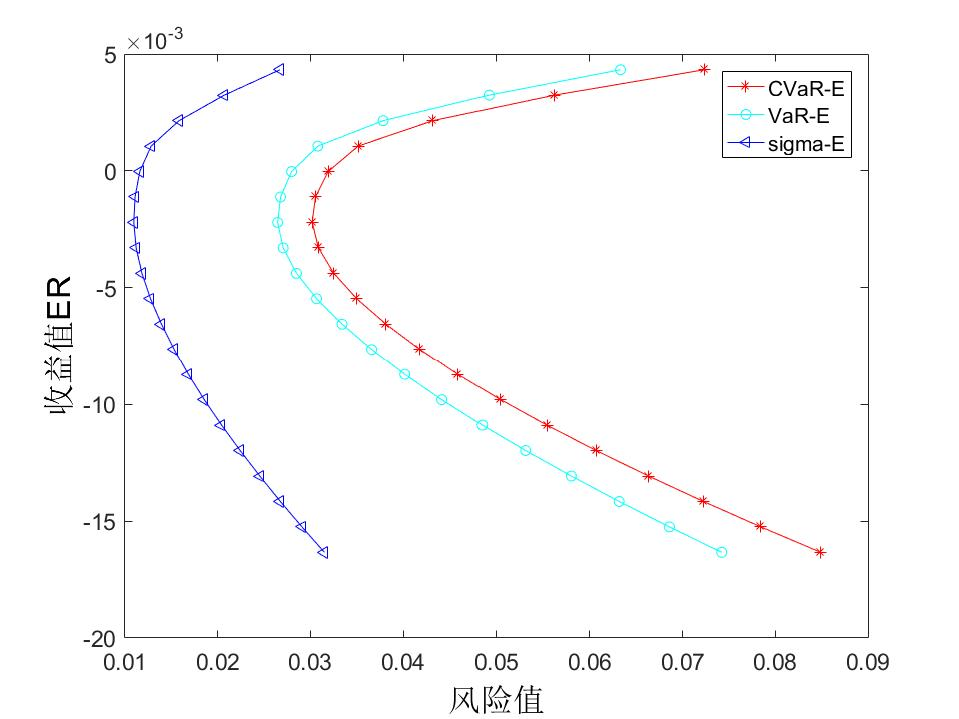
\includegraphics[width = 8cm ]{images/youxiaoqianyan.jpg}
        \caption{$t=889$各种组合模型的有效前沿}
        \label{各种组合模型的有效前沿}
        \end{figure}
        \par
        虽然在上面我们选取了时间$t=889$作为观察对象,但$t=889$可能不是最好的投资时间,我们可以规定在某一风险值下(即我们所能承受的最大风险),我们要获得最大收益$ER_t$,为此,我们需要选取最佳投资时间$t$:在$t$时刻下,在规定的风险值下,我们的收益$ER$最大。由于我们的时间跨度很大:从1-889,我们没有必要所有时间点$t$都进行研究,那样的工作量将会很大,我们以5为步长观察1到889时刻的每个时点的有效前沿,得到的结果如图(\ref{各时点t的不同组合投资模型的有效前沿})所示,从中我们看到,在时间$t=46$时,它的有效前沿异于其它时点,在同样的风险水平下,它的收益要明显高于其它时点,所以可以大致判断最优投资时间在$t=46$左右。
        \begin{figure}[H]
        \centering
        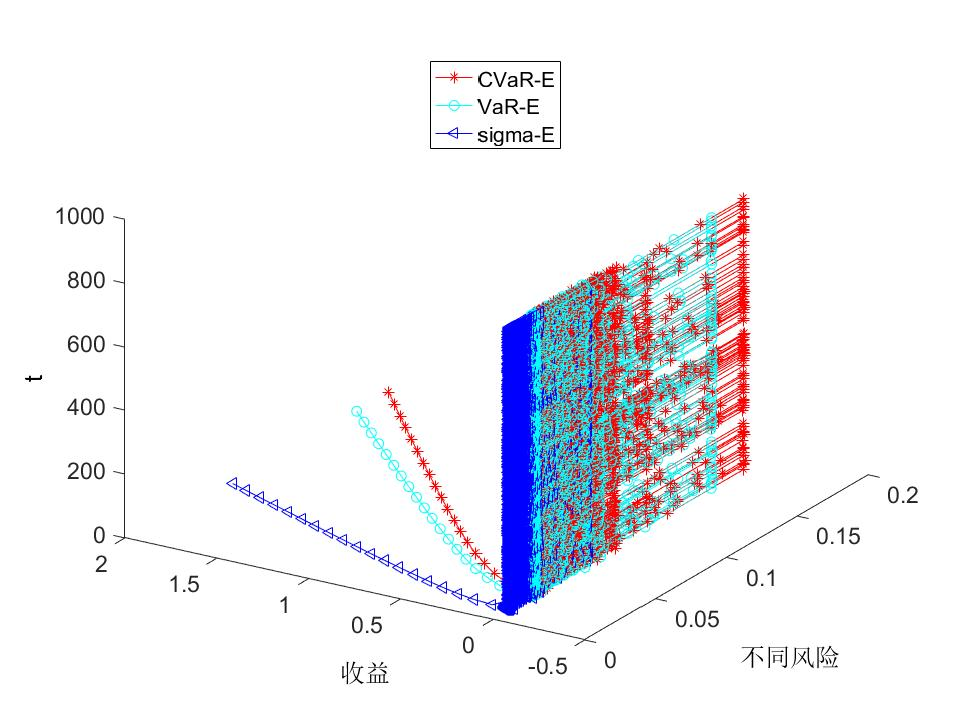
\includegraphics[width = 8cm]{images/t-cvar.jpg}
        \caption{各时点$t$的不同组合投资模型的有效前沿}
        \label{各时点t的不同组合投资模型的有效前沿}
        \end{figure}
        \par
        在最终进行求解最优投资时间和投资权重时,我们仅仅是查看了不同时点的有效前沿,选取了最优投资时间$t=46$,实际上,我们可以利用IENSGA\rom{2}算法求出具体的最优时间$t$和最优投资权重$w_i$,由于时间和篇幅原因,我们没有做相应的处理。文中模型的另一个不足之在于收益率模型,从表(\ref{9个收益率模型的信息})中我们可以看到,仍有部分模型产生的残差是具有ARCH效应的,这使得我们有必要考虑建立新的收益率模型。

% \end{document}
